\chapter{Metodología}
\label{chap:metodologia}

\drop{E}n este capítulo se va a exponer la metodología elegida para el desarrollo de este trabajo fin de grado. Se ha decidido escoger \textit{Scrum}, una metodología ágil para la gestión de proyectos.

\section{Scrum}
Scrum \cite{Schwaber2017} es un marco de trabajo de procesos que se usa para la gestión del desarrollo de productos dentro del cual se pueden emplear diferentes procesos y técnicas. Posee equipos autogestionados con sus roles, eventos, artefactos y reglas asociadas. Scrum se basa en dividir el proyecto en diferentes fases, de manera que una fase no puede comenzar mientras la anterior no haya terminado. Por tanto, en cada una de estas fases se intenta predecir qué va a pasar en la siguiente.

\subsection{Teoría de Scrum}
Scrum se basa en la teoría de control de procesos empírica, lo que asegura que el conocimiento procede de la experiencia de la toma de decisiones basadas en lo que ya se conoce empleando un enfoque iterativo e incremental. Sus tres pilares fundamentales son \cite{Schwaber2017}:

\begin{itemize}
	\item \textbf{Transparencia}. Los aspectos significativos del proceso han de ser visibles para los responsables del resultado.
	\item \textbf{Inspección}. Los usuarios de Scrum deben inspeccionar con frecuencia los artefactos y el progreso para detectar variaciones indeseadas. Estas inspecciones no deben interferir en el trabajo.
	\item \textbf{Adaptación}. Si un inspector determina que uno o más aspectos de un proceso se desvían de ciertos límites y que el resultado será inaceptable, se procederá a un reajuste que deberá realizarse tan pronto como sea posible para minimizar una desviación mayor.
\end{itemize}

Del mismo modo, se definen cuatro eventos contenidos dentro del Sprint, que serán explicados más adelante: \textbf{planificación del sprint} (\textit{Sprint Planning}), \textbf{scrum diario} (\textit{Daily Scrum}), \textbf{revisión del sprint} (\textit{Sprint Review}) y \textbf{retrospectiva del sprint} (\textit{\mbox{Sprint Retrospective}}).

\subsection{El equipo de Scrum}
Cada equipo de Scrum \cite{Schwaber2017} se compone del \textbf{dueño del producto}, \textbf{el equipo de desarrollo} y un \textbf{\textit{Scrum Master}}. Los equipos son autoorganizados y multifuncionales.

\subsection*{Dueño del producto (\textit{Product Owner})}
Es el responsable de maximizar el valor del producto desde el punto de vista del negocio. Además, es la única persona responsable de controlar el \textit{Product Backlog}, lo que incluye tareas como la de fijar sus ítems, ordenarlos, optimizar el valor del trabajo del equipo de desarrollo o asegurar que dicho equipo entiende cada ítem al nivel necesario. El dueño del producto es el responsable último de todas las tareas anteriores y el resto del equipo ha de respetar sus decisiones.

\subsection*{Equipo de desarrollo (\textit{Development Team})}
Este equipo está formado por profesionales que entregan un incremento del producto terminado que se puede poner en producción al final de cada sprint. El equipo de desarrollo tiene las siguientes características:

\begin{itemize}
	\item \textbf{Son autoorganizados}. Nadie puede indicar cómo convertir el \textit{product backlog} en incrementos.
	\item \textbf{Son multifuncionales}.
	\item \textbf{No se reconocen títulos individuales}.
	\item \textbf{No se reconocen subequipos}.
	\item \textbf{Cada miembro debe tener habilidades especializadas y áreas en las que enfocarse.}
\end{itemize}

\subsection*{\textit{Scrum Master}}
El \textit{Scrum Master} \cite{Gomez2017} es el responsable de que Scrum se entienda y se adopte y de que el equipo sea productivo. Principalmente, es un <<facilitador>>. Trabaja muy cerca del dueño del producto y del equipo y es el supervisor del \textit{Backlog}, asegurándose de que todas las historias estén correctamente descritas, priorizadas y estimadas.

\subsection{Eventos de Scrum}
Existen eventos \cite{Schwaber2017} predefinidos cuyo fin es crear regularidad y minimizar necesidad de realizar reuniones no definidas. Cada evento es un bloque de tiempo con una duración máxima.

\newpage

\subsubsection{El Sprint}
Es un bloque de tiempo de un mes o menos donde se crea un incremento del producto. Un nuevo Sprint comienza inmediatamente después de la conclusión del anterior y una de sus principales características es que, en cada uno, se solapan todas las etapas de la creación de un producto. Es decir, en cada iteración se realiza la planificación, análisis, creación y comprobación del entregable.

El Sprint tiene una serie de etapas, que son la \textbf{Planificación del Sprint} (\textit{Sprint Planning}), \textbf{Scrums Diarios} (\textit{Daily Scrums}) el \textbf{trabajo de desarrollo}, la \textbf{Revisión del Sprint} (\textit{Sprint Review}) y la \textbf{Retrospectiva del Sprint} (\textit{Sprint Retrospective}).

\subsubsection{Planificación del Sprint (\textit{Sprint Planning})}
Esta tarea se realiza al comienzo de cada Sprint, donde se planifica el trabajo a realizar \cite{Gomez2017}. Antes, el dueño del producto revisa el \textit{Product Backlog} se corresponde con las historias de usuario que le gustaría ver en la siguiente iteración, junto con su correcta descripción y priorización.

La reunión debe terminar con unos objetivos: una lista de historias o \textit{Sprint Backlog} (conjunto de historias de usuario y tareas en las que se dividen); un propósito para el Sprint que sugiere el dueño del producto; el compromiso del equipo de realizar las historias; la estimación del equipo del esfuerzo necesario para realizar cada historia; y que todos entiendan el contenido y el alcance de todas las historias.

\subsubsection{Scrum diario (\textit{Daily Meeting})}
El Scrum diario \cite{Schwaber2017} es una reunión de corta duración para la sincronización de las actividades y creación del plan de actividades por parte del equipo de desarrollo.

\subsubsection{Revisión del Sprint (\textit{Sprint Review})}
Esta tarea se realiza al final de cada Sprint para inspeccionar el incremento y adaptar el \textit{Product Backlog} si fuera necesario. Participan el equipo Scrum y los interesados en una reunión informal.

\subsubsection{Retrospectiva del Sprint (\textit{Sprint Retrospective})}
Aquí el equipo Scrum se inspecciona a sí mismo para crear un plan de mejoras para el siguiente Sprint. Se realiza después de la revisión y antes de la siguiente planificación.

\newpage

\subsection{Artefactos de Scrum}
Los artefactos \cite{Schwaber2017} representan trabajo o valor en diversas formas.

\subsubsection{Lista de Producto (\textit{Product Backlog})}
El \textit{Product Backlog} es uno de los elementos fundamentales, siendo una lista de todo lo que podría ser necesario en el producto. Contiene las características, funcionalidades, requisitos, mejoras y correcciones que conforman cambios a realizar sobre el producto para entregas futuras. Su responsable es el dueño del producto, incluyendo su contenido, disponibilidad y ordenación. Esta lista va evolucionando a medida que el producto y el entorno en el que se usará también lo hacen. Esto quiere decir que es dinámica, cambiando constantemente.

\subsubsection{Lista de Sprint (\textit{Sprint Backlog})}
Esta lista \cite{Gomez2017} contiene los trabajos a realizar en un Sprint determinado. Contiene las historias de usuario y las tareas identificadas por parte del equipo de desarrollo, que es quien gestiona esta lista. Al igual que la lista de producto, es dinámica y se va modificando durante el Sprint según se trabaja en lo planeado.

\subsubsection{Incremento}
El Incremento \cite{Schwaber2017} es la suma de todos los elementos de la lista de producto completados durante un Sprint y el valor de los Sprints anteriores.

\newpage

\section{Kanban en GitHub}
GitHub ofrece una pestaña para cada repositorio llamada \textit{projects} en la que se pueden crear tableros Kanban, que serán útiles durante el desarrollo del trabajo. Kanban \cite{Gomez2017} es una palabra de origen japonés que significa signo, señal o tarjeta. Este tablero resulta de gran ayuda puesto que se pueden observar de un rápido vistazo las tareas que quedan por hacer, en las que se está trabajando y las terminadas de una manera visual, organizada y rápida \ref{fig:kanban}.

\begin{figure}[!h]
	\begin{center}
		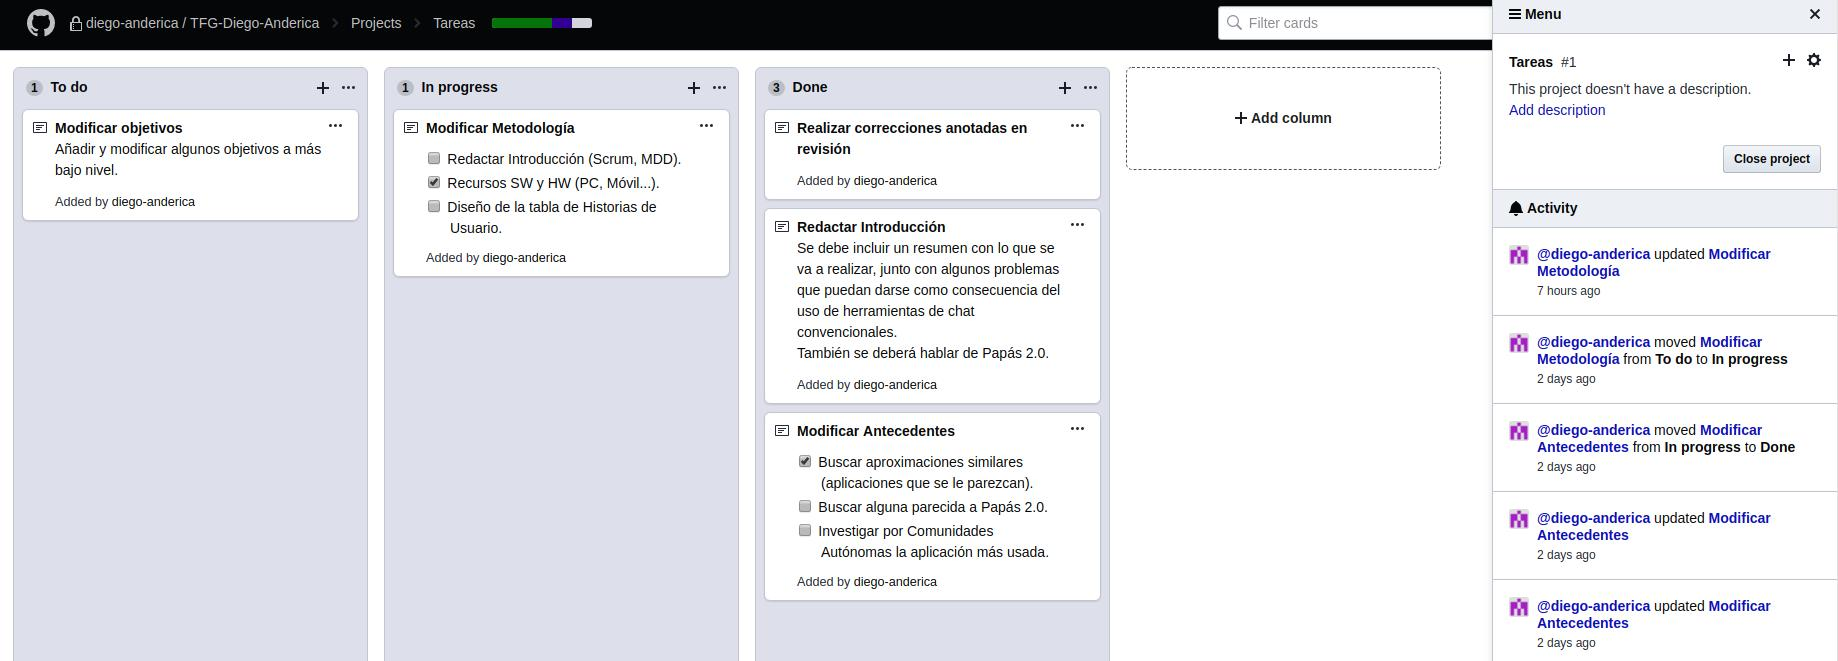
\includegraphics[width=1\textwidth]{/captura_kanban.jpg}
		\caption{Tablero Kanban en GitHub}
		\label{fig:kanban}
	\end{center}
\end{figure}